% This is a sample document using the University of Minnesota, Morris, Computer Science
% Senior Seminar modification of the ACM sig-alternate style. Much of this content is taken
% directly from the ACM sample document illustrating the use of the sig-alternate class. Certain
% parts that we never use have been removed to simplify the example, and a few additional
% components have been added.

% See https://github.com/UMM-CSci/Senior_seminar_templates for more info and to make
% suggestions and corrections.

\documentclass{sig-alternate}
\usepackage{color}
\usepackage[colorinlistoftodos]{todonotes}
\usepackage{algorithm2e}

%%%%% Uncomment the following line and comment out the previous one
%%%%% to remove all comments
%%%%% NOTE: comments still occupy a line even if invisible;
%%%%% Don't write them as a separate paragraph
%\newcommand{\mycomment}[1]{}

\begin{document}

% --- Author Metadata here ---
%%% REMEMBER TO CHANGE THE SEMESTER AND YEAR AS NEEDED
\conferenceinfo{UMM CSci Senior Seminar Conference, December 2017}{Morris, MN}

\title{Thread Scheduler Efficiency Improvements for Multiprocessor Multicore Systems [Draft]}

\numberofauthors{1}

\author{
% The command \alignauthor (no curly braces needed) should
% precede each author name, affiliation/snail-mail address and
% e-mail address. Additionally, tag each line of
% affiliation/address with \affaddr, and tag the
% e-mail address with \email.
\alignauthor
Daniel C. Frazier\\
	\affaddr{Division of Science and Mathematics}\\
	\affaddr{University of Minnesota, Morris}\\
	\affaddr{Morris, Minnesota, USA 56267}\\
	\email{frazi177@morris.umn.edu}
}
\maketitle

\todo[inline]{This is an incomplete Draft}

\begin{abstract}
[Abstract text]
\end{abstract}

\keywords{Scheduling; thread migration; multicore; multiprocessing; lock contention; last-level cache misses}

\section{Introduction}
\label{sec:intro}

Thread scheduling is a problem that has been around since the 1960's. In the 2000's the problem was considered solved but with the emergent popularity of multiprocessor multicore systems the problem space has become considerable more complex. This paper will describe some issues currently present in the Linux scheduler as well as three recent developments that substantially improve the efficiency of average programs but for certain programs improves efficiency by up to 138 times.

\section{Background}
\label{sec:bg}

In this Section we will broadly establish how threading, scheduling and caching works. We will establish causes of cache misses in the execution of programs mediated by the current implementation of thread scheduler written for Linux. We will establish information necessary to understand the recent developments made to improve thread scheduling for multiprocessor multicore non-uniform memory access systems. The first method/solution to these performance problems depend on understanding three flaws in the current implementation of the load balancer for the Linux thread scheduler. The other two solutions depend on reducing lock contention between threads via scheduling.

\subsection{Threads and Scheduling}
\label{sec:threads}
Using any modern computer, there is an expectation that the operating system is running at all times (largely in the background) and that multiple different user programs and system programs should be able to run concurrently. Modern computer programs also often need to run more than one independent task at one time. This can be accomplished by employing \emph{threads}, or equivalently, making the program \emph{multithreaded}. Programs that involve long independent computations or programs with a graphical interface often benefit from employing threads.

For an example, in the case of image editing software, say you are working on a large picture and decide to perform an expensive filtering operation. If the program wasn't multithreaded, the user interface and the filter operation would be executed in the same thread (same \emph{context}). When you instruct the program to execute the filter, the user interface wouldn't be able to respond to any events (like clicking the mouse) until the filter operation was finished. To make the program more responsive, separate the user interface into its own thread and employ more threads when the user initiates an expensive function.
	
Threads are tied to the processes that spawn them. A process always has at least one thread. Processes are typically independant of each other while threads exist within a process. \emph{Context switching} within a CPU is the process of storing and restoring the state of a process or thread so that execution can be paused or resumed.~\cite{WikiContext}. Context switching is typically faster for threads than processes because most of the state information between threads in a process is the same~\cite{WikiThreads}. 

The scheduler is the part of the operating system that is responsible for managing and distributing the CPU runtime that each of these processes and their respective threads receive. New threads and processes are added to the scheduler when they are made~\cite{Lozi:2016}.

\subsection{Completely Fair Scheduler (CFS)}
\label{sec:cfs}

Scheduler implementations vary per operating system. The scheduler used in Linux is called the Completely Fair Scheduler (CFS.) We will discuss the CFS as presented in Lozi et al.~\cite{Lozi:2016}. The CFS is an implementation of the weighted fair queuing (WFQ) scheduling algorithm. The goal of the WFQ is to divide available CPU cycles among threads, prioritizing more cycles for threads with larger weights.

Threads that are running accumulate \emph{vruntime}, which is the runtime of a thread divided by it's weight. Once a thread's vruntime is greater than the amount of runtime that the thread was scheduled for and there is another thread waiting to take this thread's place, the running thread is preempted from the CPU. A thread may also become preempted if another thread with a smaller vruntime awakens. Threads are organized in a red-black tree called a \emph{runqueue} in which the leftmost node is always the thread with the smallest vruntime.~\cite{Lozi:2016}

In order for scheduler to work on multiple cores, each core must have it's own runqueue. If all cores shared one runqueue, each core would need to frequently make expensive calls for thread context information from other cores.~\cite{Lozi:2016}. For the scheduler to function properly and efficiently, it must keep each of the runqueues balanced to minimize expensive external calls and maximize the use of available cores. Most schedulers, including the CFS, run a load balancing algorithm that tries its best to keep runqueues balanced. Load balancing was simple for single-core systems but with multi-core systems, bugs have found there way into the system and persist even until today as illustrated in the following quote:

\begin{quote}
Our recent experience with the Linux scheduler revealed that the pressure to work around the challenging properties of modern hardware, such as non-uniform memory access latencies (NUMA), high costs of cache coherency and synchronization, and diverging CPU and memory latencies, resulted in a scheduler with an incredibly complex implementation. As a result, the very basic function of the scheduler, which is to make sure that runnable threads use idle cores, fell through the cracks.~\cite{Lozi:2016}
\end{quote}

Before we can meaningfully discuss these bugs however, we must first understand how cache exists on most multiprocessor multicore systems and some related system concepts.

\subsection{Cache on NUMA Systems}
\label{sec:cache}

When a program is running, memory is stored in the RAM. The RAM exists a far ways away from the CPU relative to the cache. Imagine we had a program that sums up one million integers and they all fit in to RAM. It would be very slow for the CPU to request from the RAM every single integer one at a time. Cache allows us to speed up this process by migrating a chunk of data that the system predicts will be used frequently and moves it from the RAM into cache.

In a \emph{non-uniform memory access (NUMA)} system  there are many levels of cache and they exist in a hierarchy. At the lowest level, is a grouping of some amount of cores that together create a \emph{NUMA node}. The size of the grouping depends on the hardware. On the machine used in Lozi et al. there were 32 cores, 8 cores per NUMA node. See Figure~\ref{fig:NUMA}.~\cite{Lozi:2016} NUMA nodes are the most atomic level of cache present on a modern computing system that employs NUMA. Systems can have many levels of cache. The \emph{last level cache (LLC)} is labeled L1 and larger cache in the hierarchy are L2, L3, etc.. NUMA nodes are L1 cache and are Last level cache. Last level cache has the fastest data lookup times from a core because it is located nearer to the CPU. If a unit of cache is not found in L1 cache, it is called an \emph{LLC cache miss} and the data is searched for in the next level of cache. If the data can not be found in any level of cache it is just called an \emph{LLC cache miss}, and external memory is consulted for the data. Moving data closer to the CPU improves \emph{locality} because it makes the data more "local" to where it needs to be. Improving locality improves performance because the system works less hard to load the data it needs.~\cite{WikiCache}

\begin{figure}
\centering
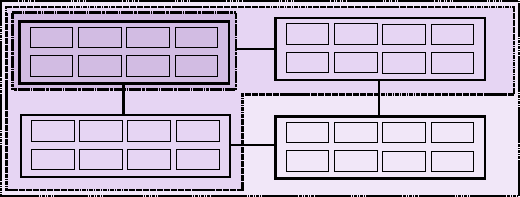
\psfig{file=NUMA.pdf,width =3in}
\caption{32-core machine with four NUMA nodes. It only takes two hops to get from any core to another node. The shades represent scheduling domains relative to the first core.  From Lozi et al.~\cite{Lozi:2016}}
\label{fig:NUMA}
\end{figure}

\subsection{Locks and Lock contention}
\label{sec:locks}

\todo[inline]{Fill out}

\section{Methods}
\label{sec:methods}

So far we've established what threads are, how cache works and where it resides on NUMA systems, how the CFS scheduler works. Now, we will discuss three bugs we found in the CFS load balancer, and their fixes which substantially improved scheduler efficiency. Later, we will show two more solutions that improve efficiency for certain kinds of programs running on multiprocessor multicore NUMA systems.

\subsection{Load Balancing the CFS}
\label{sec:loadbalance}

As we mentioned in Section \ref{sec:cfs}, modifications were made to the CFS that introduced bugs that caused processors to remain idle even when there were threads available. Work by Lozi et al. has identified four bugs that were responsible for this behaviour. These bugs have remained hidden because while they corrode performance, they aren't obvious. They don't make programs freeze or crash and their effects only last a few hundred milliseconds at a time which is too short for common performance tools like \textbf{top} to detect. Lozi et al. designed new tools that observe the linux scheduler more closely. Using these tools helped these researches locate the problems.~\cite{Lozi:2016}

In order to understand these bug fixes, as described in Lozi et al., we must explain a simplified version of the CFS load balancer.~\cite{Lozi:2016}

\subsubsection{Load Metric}
\label{sec:loadmetric}

The load balancing algorithm tracks a metric called \emph{load} to best distribute threads to cores. Defining what load should be is tricky. Balancing load such that each core has the same amount of threads is not ideal because threads have priorities, and if all of the high priority threads happened to be placed on one core while all low priority threads were placed on another, the low priority threads would be receiving much more runtime than they should be relative to the high priority threads. Balancing load such that each core has roughly the same amount of weights is not ideal either because if there was one thread that was nine times more important than nine low priority threads, that important thread would be left on a core all alone. That seems acceptable, but consider if that high priority thread sleeps a lot. It's core would be idle that whole time and would need to ask other cores for more work to keep busy in the downtime which is an expensive operation.~\cite{Lozi:2016}

The current implementation of CFS uses a combination of a thread's weights and average CPU use divided by the amount of all threads in the parent process for the load metric. It divides by the amount of all threads in the parent process in order to remain fairness so that two processes that have different amounts of threads of the same priority still get equal runtime.~\cite{Lozi:2016}

\subsubsection{Load Balancing Algorithm}
\label{sec:loadbalancealg}

Cores exist in the hierarchy where each level is called a \emph{scheduling domain}. The groups within each level are based on how cores share resources with the machine. The lowest level of scheduling domain is a single core. In the machine previously described in Section~\ref{sec:cache} there were 32 cores (first level), 4 NUMA nodes (second level), the third level was formed by groupings of nodes that are within 1 hop of eachother, and the final level is all of the nodes as one unit.
The Load balancing algorithm is run for each scheduling domain starting at the first level's scheduling domain and ending on the final level's scheduling domain. One core per scheduling domain is responsible for performing the load balancing for that domain.

\todo[inline]{finish}

\subsection{Bugs and Fixes for the CFS}
\label{sec:cfsbugs}

Now that we know how the load balancer functions, we will now dive into the bugs that occur as a result of the complex, strict requirements that have built up over time on the CFS.

\subsubsection{The Group Imbalance bug}
\label{sec:cfsfault_grpimbalance}

This bug was first encountered in the wild when the researchers were compiling the Linux kernel with \textbf{make} on 64 cores and also had two R programs running, each of which was launched from different ssh connections on 3 different ttys.

\todo[inline]{I've only just realized that Lozi doesn't mention locks or lock contention. This is interesting. I believe then that the solutions to the bugs found in Lozi are more general use case efficiency improvements to the standard CFS and the new developments I intended to write about in the METHODS section specifically optimize problems that utilize parallel programming practices (because they use locks more frequently). These are two related, but different, problems. Lozi does include a solution to the problems that they found, and so PERHAPS I should cut out one of the sections that I have not yet completed in Methods and replace it with the solutions proposed in Lozi. I need to read further and discuss this. Also, since Lozi doesn't mention lock contention, I will need to find another way to fit it in to the background section."}
\todo[inline]{I have restructured my paper as such, the results and problems from Lozi are interesting.}

~\cite{Lozi:2016}

\subsubsection{The Scheduling Group Construction bug}
\label{sec:cfsfault_grpconstruct}



\subsubsection{The Overload-on-Wakeup bug}
\label{sec:cfsfault_overload}

\subsubsection{The Missing Scheduling Domains bug}
\label{sec:cfsfault_missingsched}

This bug is actually something that was already fixed but regressed on Linux kernel version 3.19 (and later) when an important line of code was removed in a refactor that causes the system to misrepresent the amount of scheduling domains that are available for assigning threads to. This ended up causing load balancing to never happen, meaning processes, subprocesses and their threads stop looking for other NUMA nodes to assign themselves to, and nodes that don't have any threads will never receive threads and nodes that do have threads will accumulate all of the spawned threads.

While rare (the bug required that one of the cores become disabled and re-enable) reintroducing the removed line of code increased efficiency in a tested program by a maximum of 138 times more efficient.~\cite{Lozi:2016}

\subsection{Shuffler}
\label{sec:shuffler}

The CFS doesn't differentiate between threads of a single-threaded program versus the threads of a multithreaded program. This prevents the scheduler from using that metadata in it's thread distribution mechanism. The following thread scheduler improve upon this.

Performance of multithreaded applications on multicore multiprocessor systems with high lock contention is dependant on the distribution of those threads across processors. The Shuffling approach is for the scheduling algorithm to take into account what threads are contending for locks on what processors and migrate threads to share processors. The Shuffling Framework does this by the following. First we find the expected arrival time of locks on threads. Then we sort these threads by their expected arrival times and group them in as many groups as there are processors. Then we distribute these groups of threads to their own respective processors. The migration of threads between processors is costly, but the threads that are contending for locks during that time are not doing any useful work anyway. In addition, contending threads that are co-located in one processor can share data much faster and avoid LLC misses. For these reasons it is preferable to migrate the whole thread rather than it's data and the lock. This will be shown in the Performance section.~\cite{KumarEtal:2014}

For the first step of the algorithm you must find the expected arrival time of threads. The \textit{lock time} of a thread is measured by the percent of time it spends waiting for locks. There exists a daemon thread that contains a data structure that maps threads to their lock times and processor ids. For the monitor we must choose a rate to sample lock acquiring times at (lock arrival times) and a rate to perform thread migration (shuffling). Kumar et al. used prstat, a utility to report active processor statistics~\cite{prstat}, to monitor lock arrival times. They found that finer sampling rates allow for detailed monitoring but also more overhead. They also found that for sampling rates less than 200 ms, the overhead was significantly higher. For a lock sampling rate of 200 ms the process of sampling took less than 1\% system time. The Shuffling interval was chosen by experimentation. They tested various shuffling intervals on 20 programs and chose 500 ms.

On an iteration of the grouping-forming procedure (every 200 ms), the daemon checks the total amount of time that was spent resolving locks on each thread and if that time exceeds a preset limit, then groups are formed again.

On an iteration of the shuffling procedure (every 500 ms), shuffling checks to make sure that if any threads aren't on processors that they were grouped to, they are migrated. Threads that are already on the processor that they were assigned to do not migrate. If the way that threads interacted with eachother doesn't change, the shuffling step is effectively skipped.~\cite{KumarEtal:2014}

\begin{algorithm}
	\SetKwInOut{Input}{input}\SetKwInOut{Output}{output}
	\Input{N: Number of threads;\\
	C: Number of Processors.}

	\Repeat{application terminates}{
		$\textbf{i. Monitor Threads}$ -- sample lock times of N threads.\\
		\If{lock times exceed threshold}{
			$\textbf{ii. Form Thread Groups}$ -- sort threads according to lock times and divide them into C groups. \\
			$\textbf{iii. Perform Shuffling}$ -- shuffle threads to establish newly computed thread groups.
		}
	}			

	\caption{The Shuffling Framework
	as presented in Kumar et al.}\label{euclid}\label{alg:shuffler}
\end{algorithm}

Now that we know how the Shuffling Framework works, let's review the results that implementing it gives us.

\subsubsection{Shuffler Performance}
\label{sec:shuf_performance}

Kumar et al. defines LLC miss rate as the last level cache misses per thousand instructions (MPKI).~\cite{KumarEtal:2014}.

We studied the lock times of 33 programs on a 64-core, 4-processor machine running Oracle Solaris 11. We identified 20 of those programs that experienced overall high lock times and used those programs to compare shuffling versus the standard scheduler.~\cite{KumarEtal:2014}

\todo[inline]{expand, relay more results! Transition cleanly.}


\subsection{FLSCHED for Xeon Phi Manycore Processor}
\label{sec:flsched}

\todo[inline]{I feel like this source is relevant because it details thread scheduler efficiency improvements for a unique multicore processor. But it is not a multiprocessor.  Multiprocessor is in the title of my paper. Should I still use this source? I think the results sound fascinating and I'm really excited to write about it. Should I adapt the title of my paper to exclude the assumption of multiproccessing? The topic should still be pretty specific even with that change.}

\todo[inline]{write section..}

[Body text]

\subsubsection{Lockless Thread Scheduler}
\label{sec:flsched_about}

\cite{Lozi:2016, NisarEtal:2017}
~\cite{KumarEtal:2014}

\subsubsection{FLSCHED Perfomance}
\label{sec:flsched_performance}

[Body text]

\section{Conclusions}
\label{sec:conclusions}

[Conclusion text]
\todo[inline]{After other sections are done write conclusions and introduction.}

\section*{Acknowledgments}
\label{sec:acknowledgments}


% The following two commands are all you need in the
% initial runs of your .tex file to
% produce the bibliography for the citations in your paper.
\bibliographystyle{abbrv}
% sample_paper.bib is the name of the BibTex file containing the
% bibliography entries. Note that you *don't* include the .bib ending here.
\bibliography{scheduling}  
% You must have a proper ".bib" file
%  and remember to run:
% latex bibtex latex latex
% to resolve all references

\end{document}
